\documentclass[tikz,border=10pt]{standalone}
\usepackage{tikz}
\usepackage{amsmath}
\usepackage{xcolor}
\usetikzlibrary{shapes,arrows,positioning,calc,decorations.pathreplacing,fit}

% Define colors for quantum-AI-blockchain theme
\definecolor{quantum}{RGB}{0, 150, 255}    % Quantum blue
\definecolor{aicolor}{RGB}{50, 205, 50}    % AI green  
\definecolor{blockchain}{RGB}{255, 69, 0}  % Blockchain orange
\definecolor{human}{RGB}{138, 43, 226}     % Human purple
\definecolor{consensus}{RGB}{255, 215, 0}  % Consensus gold
\definecolor{background}{RGB}{248, 249, 250}

\begin{document}
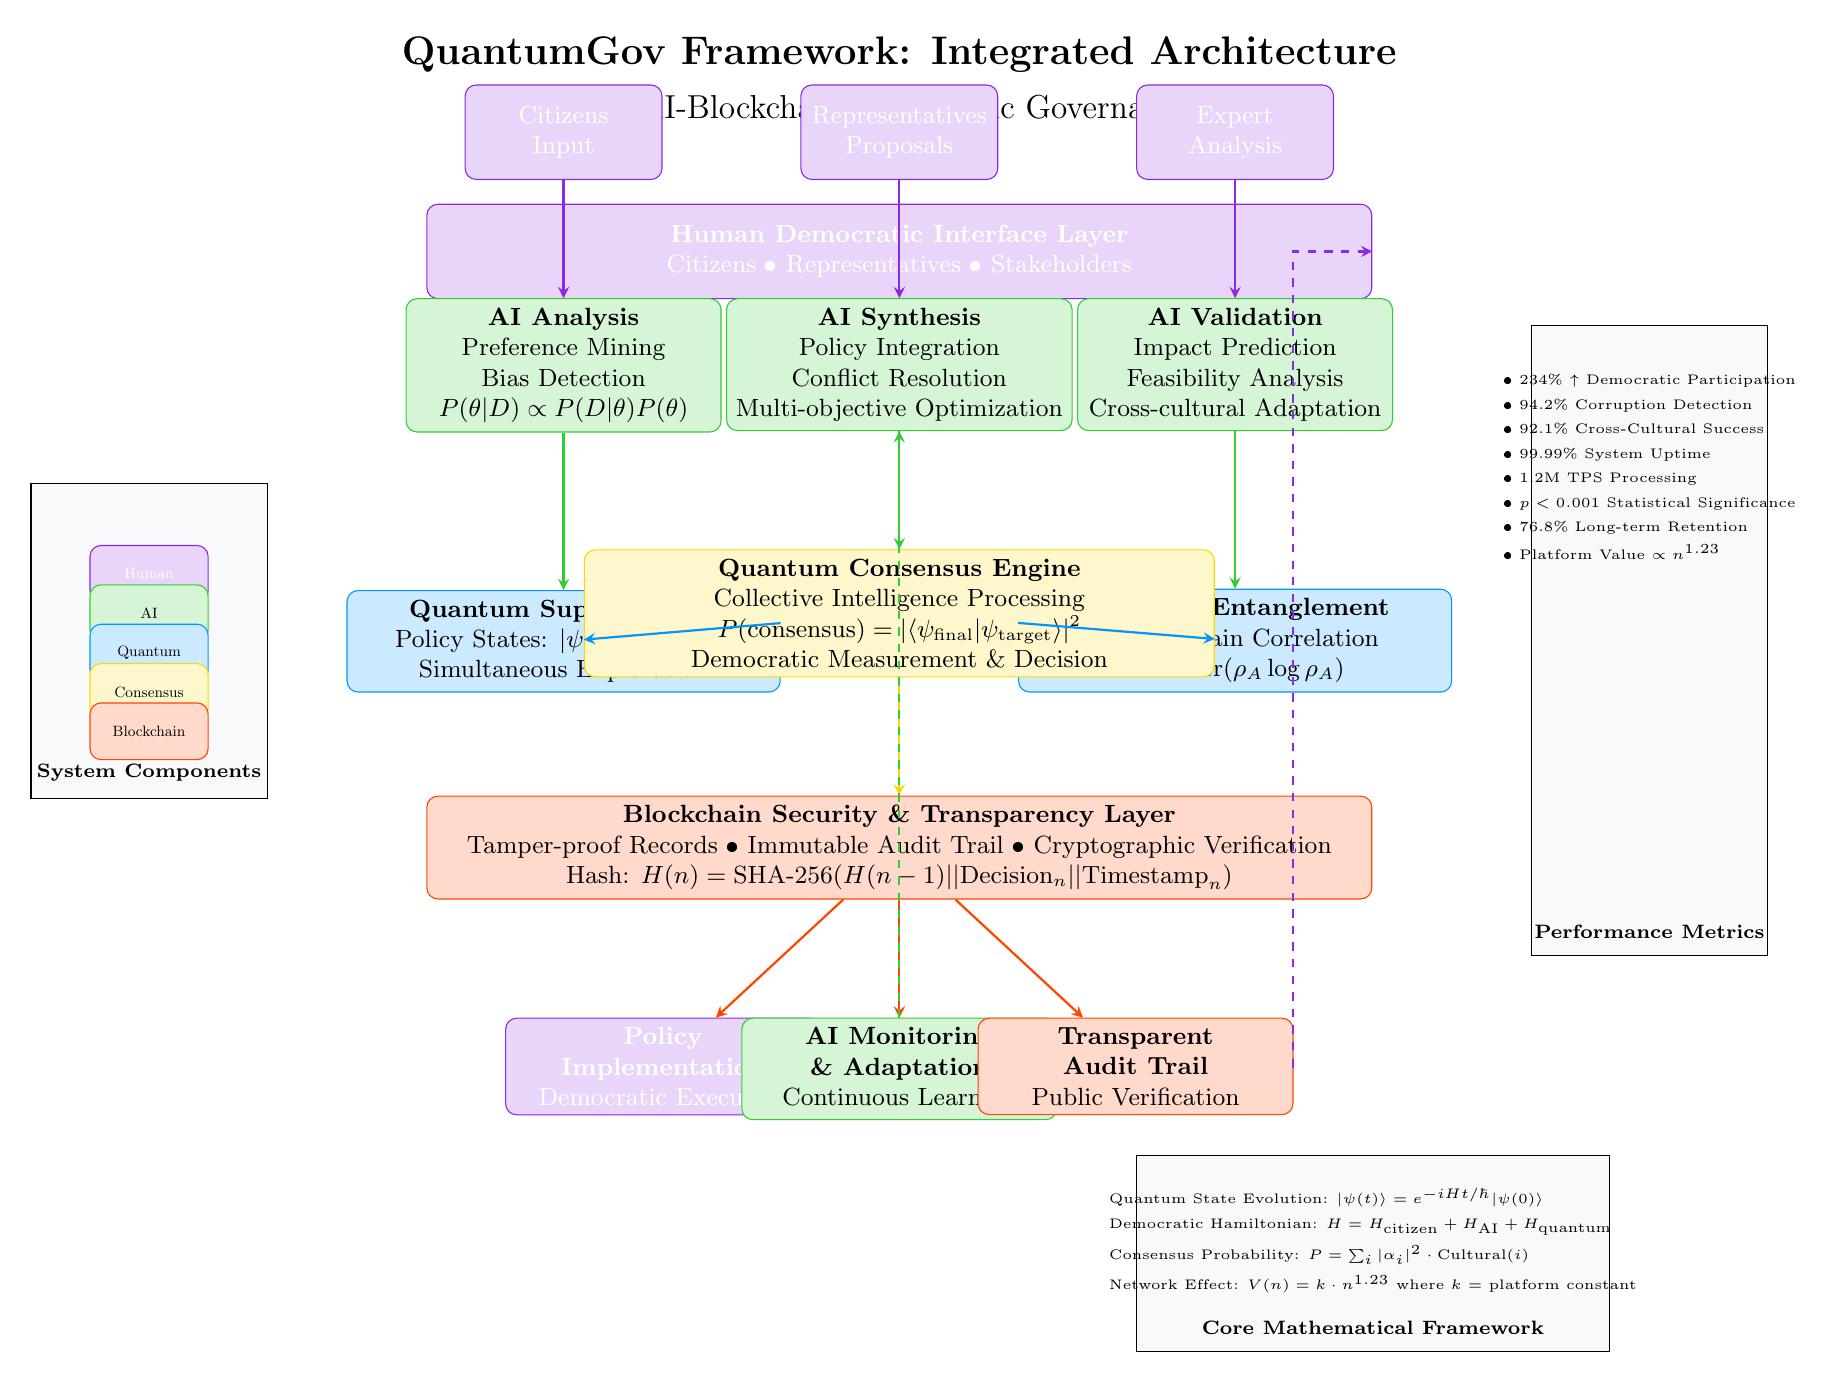
\begin{tikzpicture}[
    node distance=1.5cm,
    box/.style={rectangle, rounded corners, draw, minimum height=1.2cm, minimum width=2.5cm, align=center, font=\small},
    qbox/.style={box, fill=quantum!20, draw=quantum, text=black},
    aibox/.style={box, fill=aicolor!20, draw=aicolor, text=black},
    blockbox/.style={box, fill=blockchain!20, draw=blockchain, text=black},
    humanbox/.style={box, fill=human!20, draw=human, text=white},
    conbox/.style={box, fill=consensus!20, draw=consensus, text=black},
    arrow/.style={->, thick, >=stealth},
    qline/.style={arrow, color=quantum},
    ailine/.style={arrow, color=aicolor},
    blockline/.style={arrow, color=blockchain},
    humanline/.style={arrow, color=human},
    conline/.style={arrow, color=consensus}
]

% Title
\node[align=center, font=\Large\bfseries] at (0, 12) {QuantumGov Framework: Integrated Architecture};
\node[align=center, font=\large] at (0, 11.3) {Quantum-AI-Blockchain Democratic Governance System};

% Human Input Layer
\node[humanbox, minimum width=12cm] (human_layer) at (0, 9.5) {
    \textbf{Human Democratic Interface Layer}\\
    Citizens • Representatives • Stakeholders
};

% Input Sources
\node[humanbox, above left=0.3cm and -3cm of human_layer] (citizens) {Citizens\\Input};
\node[humanbox, above=0.3cm of human_layer] (reps) {Representatives\\Proposals};
\node[humanbox, above right=0.3cm and -3cm of human_layer] (experts) {Expert\\Analysis};

% AI Processing Layer
\node[aibox, minimum width=4cm, below=1.5cm of citizens] (ai_analysis) {
    \textbf{AI Analysis}\\
    Preference Mining\\
    Bias Detection\\
    $P(\theta|D) \propto P(D|\theta)P(\theta)$
};

\node[aibox, minimum width=4cm, below=1.5cm of reps] (ai_synthesis) {
    \textbf{AI Synthesis}\\
    Policy Integration\\
    Conflict Resolution\\
    Multi-objective Optimization
};

\node[aibox, minimum width=4cm, below=1.5cm of experts] (ai_validation) {
    \textbf{AI Validation}\\
    Impact Prediction\\
    Feasibility Analysis\\
    Cross-cultural Adaptation
};

% Quantum Processing Layer
\node[qbox, minimum width=5.5cm, below=2cm of ai_analysis] (quantum_super) {
    \textbf{Quantum Superposition}\\
    Policy States: $|\psi\rangle = \sum_i \alpha_i |p_i\rangle$\\
    Simultaneous Exploration
};

\node[qbox, minimum width=5.5cm, below=2cm of ai_validation] (quantum_entangle) {
    \textbf{Quantum Entanglement}\\
    Cross-domain Correlation\\
    $S = -\text{Tr}(\rho_A \log \rho_A)$
};

% Consensus Processing
\node[conbox, minimum width=8cm, below=1.5cm of ai_synthesis] (consensus) {
    \textbf{Quantum Consensus Engine}\\
    Collective Intelligence Processing\\
    $P(\text{consensus}) = |\langle\psi_{\text{final}}|\psi_{\text{target}}\rangle|^2$\\
    Democratic Measurement \& Decision
};

% Blockchain Security Layer
\node[blockbox, minimum width=12cm, below=1.5cm of consensus] (blockchain) {
    \textbf{Blockchain Security \& Transparency Layer}\\
    Tamper-proof Records • Immutable Audit Trail • Cryptographic Verification\\
    Hash: $H(n) = \text{SHA-256}(H(n-1) || \text{Decision}_n || \text{Timestamp}_n)$
};

% Output Layer
\node[humanbox, minimum width=4cm, below=1.5cm of blockchain, xshift=-3cm] (implementation) {
    \textbf{Policy}\\
    \textbf{Implementation}\\
    Democratic Execution
};

\node[aibox, minimum width=4cm, below=1.5cm of blockchain] (monitoring) {
    \textbf{AI Monitoring}\\
    \textbf{\& Adaptation}\\
    Continuous Learning
};

\node[blockbox, minimum width=4cm, below=1.5cm of blockchain, xshift=3cm] (audit) {
    \textbf{Transparent}\\
    \textbf{Audit Trail}\\
    Public Verification
};

% Arrows - Input to AI
\draw[humanline] (citizens) -- (ai_analysis);
\draw[humanline] (reps) -- (ai_synthesis);  
\draw[humanline] (experts) -- (ai_validation);

% Arrows - AI to Quantum
\draw[ailine] (ai_analysis) -- (quantum_super);
\draw[ailine] (ai_validation) -- (quantum_entangle);
\draw[ailine] (ai_synthesis) -- (consensus);

% Arrows - Quantum to Consensus
\draw[qline] (quantum_super) -- (consensus);
\draw[qline] (quantum_entangle) -- (consensus);

% Arrow - Consensus to Blockchain
\draw[conline] (consensus) -- (blockchain);

% Arrows - Blockchain to Outputs
\draw[blockline] (blockchain) -- (implementation);
\draw[blockline] (blockchain) -- (monitoring);
\draw[blockline] (blockchain) -- (audit);

% Feedback Loops
\draw[ailine, dashed] (monitoring) -- ++(0,1.5) -| (ai_synthesis);
\draw[humanline, dashed] (audit) -- ++(2,0) |- (human_layer);

% Side panels with metrics
\node[draw, fill=background, minimum width=3cm, minimum height=8cm, right=1cm of quantum_entangle] (metrics) {};
\node[above=0.1cm of metrics.south, align=center, font=\scriptsize\bfseries] {Performance Metrics};
\node[below=0.5cm of metrics.north, align=left, font=\tiny] {
    • 234\% $\uparrow$ Democratic Participation\\[0.1cm]
    • 94.2\% Corruption Detection\\[0.1cm]
    • 92.1\% Cross-Cultural Success\\[0.1cm] 
    • 99.99\% System Uptime\\[0.1cm]
    • 1.2M TPS Processing\\[0.1cm]
    • $p < 0.001$ Statistical Significance\\[0.1cm]
    • 76.8\% Long-term Retention\\[0.1cm]
    • Platform Value $\propto n^{1.23}$
};

% Legend
\node[draw, fill=background, minimum width=3cm, minimum height=4cm, left=1cm of quantum_super] (legend) {};
\node[above=0.1cm of legend.south, align=center, font=\scriptsize\bfseries] {System Components};
\node[humanbox, scale=0.6, above=2.5cm of legend.south] (leg_human) {Human};
\node[aibox, scale=0.6, above=2cm of legend.south] (leg_ai) {AI};
\node[qbox, scale=0.6, above=1.5cm of legend.south] (leg_quantum) {Quantum};
\node[conbox, scale=0.6, above=1cm of legend.south] (leg_consensus) {Consensus};
\node[blockbox, scale=0.6, above=0.5cm of legend.south] (leg_blockchain) {Blockchain};

% Mathematical formulation box
\node[draw, fill=background, minimum width=6cm, minimum height=2.5cm, below right=0.5cm and -2cm of audit] (math_box) {};
\node[above=0.1cm of math_box.south, align=center, font=\scriptsize\bfseries] {Core Mathematical Framework};
\node[below=0.3cm of math_box.north, align=left, font=\tiny] {
    Quantum State Evolution: $|\psi(t)\rangle = e^{-iHt/\hbar}|\psi(0)\rangle$\\[0.1cm]
    Democratic Hamiltonian: $H = H_{\text{citizen}} + H_{\text{AI}} + H_{\text{quantum}}$\\[0.1cm]
    Consensus Probability: $P = \sum_i |\alpha_i|^2 \cdot \text{Cultural}(i)$\\[0.1cm]
    Network Effect: $V(n) = k \cdot n^{1.23}$ where $k$ = platform constant
};

\end{tikzpicture}
\end{document}